\documentclass[12pt]{article}

\usepackage{amsmath, mathtools}
\usepackage{amsfonts}
\usepackage{amssymb}
\usepackage{graphicx}
\usepackage{colortbl}
\usepackage{xr}
\usepackage{hyperref}
\usepackage{longtable}
\usepackage{xfrac}
\usepackage{tabularx}
\usepackage{float}
\usepackage{siunitx}
\usepackage{booktabs}
\usepackage{caption}
\usepackage{pdflscape}
\usepackage{afterpage}
\usepackage{titlesec}
\usepackage{graphicx}
\usepackage{enumitem}
\usepackage[round]{natbib}

%\usepackage{refcheck}

\hypersetup{
    bookmarks=true,         % show bookmarks bar?
     colorlinks=true,       % false: boxed links; true: colored links
    linkcolor=red,          % color of internal links (change box color with linkbordercolor)
    citecolor=green,        % color of links to bibliography
    filecolor=magenta,      % color of file links
    urlcolor=cyan           % color of external links
}

%% Comments

\usepackage{color}

\newif\ifcomments\commentstrue %displays comments
%\newif\ifcomments\commentsfalse %so that comments do not display

\ifcomments
\newcommand{\authornote}[3]{\textcolor{#1}{[#3 ---#2]}}
\newcommand{\todo}[1]{\textcolor{red}{[TODO: #1]}}
\else
\newcommand{\authornote}[3]{}
\newcommand{\todo}[1]{}
\fi

\newcommand{\wss}[1]{\authornote{blue}{SS}{#1}} 
\newcommand{\plt}[1]{\authornote{magenta}{TPLT}{#1}} %For explanation of the template
\newcommand{\an}[1]{\authornote{cyan}{Author}{#1}}

%% Common Parts

\newcommand{\progname}{ProgName} % PUT YOUR PROGRAM NAME HERE
\newcommand{\authname}{Team \#, Team Name
\\ Student 1 name
\\ Student 2 name
\\ Student 3 name
\\ Student 4 name} % AUTHOR NAMES                  

\usepackage{hyperref}
    \hypersetup{colorlinks=true, linkcolor=blue, citecolor=blue, filecolor=blue,
                urlcolor=blue, unicode=false}
    \urlstyle{same}
                                


% For easy change of table widths
\newcommand{\colZwidth}{1.0\textwidth}
\newcommand{\colAwidth}{0.13\textwidth}
\newcommand{\colBwidth}{0.82\textwidth}
\newcommand{\colCwidth}{0.1\textwidth}
\newcommand{\colDwidth}{0.05\textwidth}
\newcommand{\colEwidth}{0.8\textwidth}
\newcommand{\colFwidth}{0.17\textwidth}
\newcommand{\colGwidth}{0.5\textwidth}
\newcommand{\colHwidth}{0.28\textwidth}

% Used so that cross-references have a meaningful prefix
\newcounter{defnum} %Definition Number
\newcommand{\dthedefnum}{GD\thedefnum}
\newcommand{\dref}[1]{GD\ref{#1}}
\newcounter{datadefnum} %Datadefinition Number
\newcommand{\ddthedatadefnum}{DD\thedatadefnum}
\newcommand{\ddref}[1]{DD\ref{#1}}
\newcounter{theorynum} %Theory Number
\newcommand{\tthetheorynum}{T\thetheorynum}
\newcommand{\tref}[1]{T\ref{#1}}
\newcounter{tablenum} %Table Number
\newcommand{\tbthetablenum}{T\thetablenum}
\newcommand{\tbref}[1]{TB\ref{#1}}
\newcounter{assumpnum} %Assumption Number
\newcommand{\atheassumpnum}{P\theassumpnum}
\newcommand{\aref}[1]{A\ref{#1}}
\newcounter{goalnum} %Goal Number
\newcommand{\gthegoalnum}{P\thegoalnum}
\newcommand{\gsref}[1]{GS\ref{#1}}
\newcounter{instnum} %Instance Number
\newcommand{\itheinstnum}{IM\theinstnum}
\newcommand{\iref}[1]{IM\ref{#1}}

\newcounter{reqnum} %Requirement Number
\newcommand{\rthereqnum}{P\thereqnum}
\newcounter{frreqnum} % Facial Recognition Requirement Number
\newcommand{\rthefrreqnum}{P\thefrreqnum}
\newcounter{hmreqnum} % Hair Modification Requirement Number
\newcommand{\rthehmreqnum}{P\thehmreqnum}
\newcounter{arreqnum} %Authentication Requirement Number
\newcommand{\rthearreqnum}{P\thearreqnum}

\newcounter{hrreqnum} % Hair Salon Requirement Number
\newcommand{\rthehrreqnum}{P\thehrreqnum}

\newcounter{aprreqnum} % Appearance Requirement Number
\newcommand{\rtheaprreqnum}{P\theaprreqnum}
\newcounter{iarreqnum} % Interface Style Requirement Number
\newcommand{\rtheiarreqnum}{P\theiarreqnum}

\newcounter{eurreqnum} % Ease of Use Requirement Number
\newcommand{\rtheeurreqnum}{P\theeurreqnum}
\newcounter{lrreqnum} % Learning Requirement Number
\newcommand{\rthelrreqnum}{P\thelrreqnum}
\newcounter{uprreqnum} % Understandability and Politeness Requirement Number
\newcommand{\rtheuprreqnum}{P\theuprreqnum}
\newcounter{asrreqnum} % Accessibility Requirement Number
\newcommand{\rtheasrreqnum}{P\theasrreqnum}

\newcounter{slrreqnum} % Speed and Latency Requirement Number
\newcommand{\rtheslrreqnum}{P\theslrreqnum}
\newcounter{parreqnum} % Precision and Accuracy Requirement Number
\newcommand{\rtheparreqnum}{P\theparreqnum}
\newcounter{rarreqnum} % Reliability and Availability Requirement Number
\newcommand{\rtherarreqnum}{P\therarreqnum}
\newcounter{rbrreqnum} % Robustness Requirement Number
\newcommand{\rtherbrreqnum}{P\therbrreqnum}
\newcounter{ccrreqnum} % Capacity Requirement Number
\newcommand{\rtheccrreqnum}{P\theccrreqnum}
\newcounter{serreqnum} % Scalablity and Extensibility Requirement Number
\newcommand{\rtheserreqnum}{P\theserreqnum}
\newcounter{lgrreqnum} % Longevity Requirement Number
\newcommand{\rthelgrreqnum}{P\thelgrreqnum}

\newcounter{pdrreqnum} % Productiontization Requirement Number
\newcommand{\rthepdrreqnum}{P\thepdrreqnum}
\newcounter{rerreqnum} % Release Requirement Number
\newcommand{\rthererreqnum}{P\thererreqnum}

\newcounter{ucnum} % Use Case Number
\newcommand{\rucnum}{P\ucnum}

\newcounter{acrreqnum} % Access Requirement Number
\newcommand{\rtheacrreqnum}{P\theacrreqnum}
\newcounter{irreqnum} % Integrity Requirement Number
\newcommand{\rtheirreqnum}{P\theirreqnum}
\newcounter{prrreqnum} % Privacy Requirement Number
\newcommand{\rtheprrreqnum}{P\theprrreqnum}
\newcounter{aurreqnum} % Audit Requirement Number
\newcommand{\rthererrreqnum}{P\thererrreqnum}
\newcounter{rerrreqnum} % release Requirement Number
\newcommand{\rtheaurreqnum}{P\theaurreqnum}
\newcounter{msrreqnum} % maintenance Requirement Number
\newcommand{\rthemsrreqnum}{P\themsrreqnum}
\newcounter{adrreqnum} % adaptability Requirement Number
\newcommand{\rtheadrreqnum}{P\theadrreqnum}
\newcounter{sprreqnum} % Supportability Requirement Number
\newcommand{\rthesprreqnum}{P\thesprreqnum}

\newcounter{crreqnum} % Cultural Requirement Number
\newcommand{\rthecrreqnum}{P\thecrreqnum}
\newcounter{cprreqnum} % Compliance Number
\newcommand{\rthecprreqnum}{P\thecprreqnum}
\newcounter{sdrreqnum} % Audit Requirement Number
\newcommand{\rthesdrreqnum}{P\thesdrreqnum}

\newcommand{\rref}[1]{R\ref{#1}}
\newcounter{nfrnum} %NFR Number
\newcommand{\rthenfrnum}{NFR\thenfrnum}
\newcommand{\nfrref}[1]{NFR\ref{#1}}
\newcounter{lcnum} %Likely change number
\newcommand{\lthelcnum}{LC\thelcnum}
\newcommand{\lcref}[1]{LC\ref{#1}}

\newlist{UC}{enumerate}{1}
\setlist[UC]{label=UC\arabic*:}

\newcounter{ulcnum} %Likely change number
\newcommand{\ltheulcnum}{ULC\theulcnum}
\newcommand{\ulcref}[1]{ULC\ref{#1}}
\usepackage{fullpage}

\newcommand{\deftheory}[9][Not Applicable]
{
\newpage
\noindent \rule{\textwidth}{0.5mm}

\paragraph{RefName: } \textbf{#2} \phantomsection 
\label{#2}

\paragraph{Label:} #3

\noindent \rule{\textwidth}{0.5mm}

\paragraph{Equation:}

#4

\paragraph{Description:}

#5

\paragraph{Notes:}

#6

\paragraph{Source:}

#7

\paragraph{Ref.\ By:}

#8

\paragraph{Preconditions for \hyperref[#2]{#2}:}
\label{#2_precond}

#9

\paragraph{Derivation for \hyperref[#2]{#2}:}
\label{#2_deriv}

#1

\noindent \rule{\textwidth}{0.5mm}

}

\begin{document}

\title{Software Requirements Specification for Hairesthetics: A 3D Hairstyle Simulation iOS App} 

\author{Team 18 \\ Charlotte Cheng
        \\ Marlon Liu
        \\ Senni Tan
        \\ Qiushi Xu
        \\ Hongwei Niu
        \\ Bill Song
}

\date{\today}
	
\maketitle

~\newpage

\pagenumbering{roman}

\tableofcontents
\listoftables
\listoffigures

\section*{Revision History}

\begin{tabularx}{\textwidth}{p{3cm}p{2cm}X}
\toprule {\bf Date} & {\bf Version} & {\bf Notes}\\
\midrule
Oct 1 & 1.0 & Initial Drafts\\
Oct 4 & 1.1 & Update template based on rubric\\
\bottomrule
\end{tabularx}

~\newpage

\pagenumbering{arabic}
  

\includegraphics{universe}

\section{Project Drivers}

\subsection{The Purpose of the Project}
  
The purpose for this document is to provide the basic requirements for a software application that helps user simulate hairstyles and hair colors virtually. It should include the essential functional requirements, which specify the behavioral capability of the system, as well as the non-functional requirements in order to create a successful and robust application. \\
\newline
\noindent
This document should also act like an agreement between the stakeholders and the developers that the design should be based on the critical information provided in this document. The requirements should be the guiding principles in the design phase to guarantee that all the requirements are met. 

\subsection{Stakeholders}
\subsubsection{User}
\item People who have the demand to change their hair style and see how other hairstyles and different hair colors match their appearance virtually are welcome to explore in this iOS application.

\subsubsection{Client}

The clients for this project with be the students from the capstone course. These individuals will review and test the software before being deployed to the general public. In addition, the teach assistants and the supervisor will be actively involved throughout
the construction of this project.

\subsubsection{Other Stakeholders}
Other stakeholder could be the hair dressers and barbers. They can provide this app for their customer to help making a hairstyle decision.

\subsubsection{User Characteristics}
The identified users of the project can be categorized into 2 distinct groups. These groups are differentiated based on their varying background, experience of the user and their intended use(s) of the system. They are classified as the novice user and administrative user. \\
\newline
\noindent
It is assumed that all system users have experience operating with iOS applications. More specifically, all users are assumed to have experience working with iPhone, iOS 14, and above. They have been exposed to the camera app and most common icons by Apple.
\begin{itemize}
    \item Novice User: The application requires no prior training, and it is meant for the public, so all non-administrative users are novice users. Their intention is to use the application to simulate hairstyles and hair colors virtually. Anyone who does not have optic disabilities and other physical disabilities that make them unable to use the application on a smartphone can use the application.
    \item Administrative User: Their intention is not to use the application to simulate hairstyles, but to calibrate, configure, and maintain the application to make sure it functions properly and to its maximal capabilities. They wish to fix bugs, maintain database, and implement new features. They have a basic knowledge of computers, data management and app development.
    
\end{itemize}

~\newpage

\section{Project Constraints}
\subsection{Mandated Constraints}
\subsubsection{Solution Constraints}
\textbf{Description}: The product shall operate using iOS 14 and above. \\
\textbf{Rationale}: The users use iOS 14 and do not want to update system. \\
\textbf{Fit Criterion}: The product shall be approved as iOS 14 compliant by developers. \\
\newline
\textbf{Description}: The product shall use the default camera system on the iphone device to obtain the input image and videos from users. \\
\textbf{Rationale}: The users will not pay for a new graphic input device. \\
\textbf{Fit Criterion}: All graphical inputs should come from the default camera with the device. \\
\subsubsection{Implementation Environment of the Current System}
\begin{itemize}
    \item Source code is entirely written in Python and swift.
    \item Backend framework Flask is used to create user login system.
    \item MongoDB is used for storing and manipulating the password database.
    \item iOS AR kit is used for developing AR components.
    \item OpenCV is mainly used for capturing and analysing user's facial feature
\end{itemize}
\subsubsection{Off-The-Shelf Software}
\begin{itemize}
    \item Facial Contour Detection API from google ML Kit.
\end{itemize}
\subsubsection{Partner or Collaborative Applications}
N/A. \\All the external libraries / API used are open-sourced and free of charge.
\subsubsection{Anticipated Workplace Environment}
The workplace could be anywhere with a visible screen and camera. When The workplace is outside, the device must be weather resistant, have displays that are visible in sunlight, and allow for the effect of surrounding environment on output.
\subsubsection{Schedule Constraints}
Project must be completed before the end of the academic year. This will limit the amount, complexity and quality of the additional features upon initial release date.
\subsubsection{Budget Constraints}
The cost of the project must not exceed \$750. This limitation will constrain the number of requirements that can be included in the project.
\subsection{Naming Conventions and Terminology}
\subsubsection{Abbreviations and Acronyms}
\begin{enumerate}
\item \textbf{UI} - User Interface
\item \textbf{GUI} - Graphical User Interface
\item \textbf{UI} - A high-level, modern programming language that is used both on the client-side and server-side.
\item \textbf{AI} - Artificial Intelligence
\item \textbf{API} - Application programming interface
\item \textbf{REST} - Representational state transfer
\item \textbf{OS} - Operating System
\item \textbf{RGB} - Red, Green, Blue

\end{enumerate}

  
\subsection{Relevant Facts and Assumptions}
\begin{itemize}
    \item Users will have access to the internet through WiFi or though their data plan from their mobile phone.
    \item Users can understand English text.
    \item Users have healthy vision and have no difficulties in seeing colors, graphs and words on the mobile screen.
\end{itemize}

\section{Functional Requirements}
\subsection{The Scope of the Work}
Many people wonder how a different hairstyle would look on them in real life. Most of them rely on their imagination and feelings, and some uses some applications with simple filters. Thus, the existing market lacks mobile applications that accurately simulate their look with a new hairstyle or color.

\subsection{The Context of the Work}
\graphicspath{ {./context_work_diagram.jpg/} }
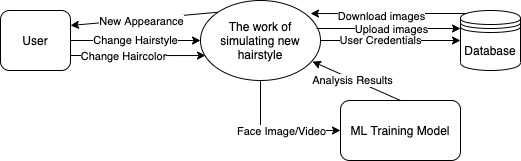
\includegraphics[width=\textwidth]{context_work_diagram}
\begin{figure}[h!]
\begin{center}
 \includegraphics[width=0.6\textwidth]{WorkContextFigure}
\caption{Context of Work Diagram}
\label{Fig_SystemContext} 
\end{center}
\end{figure}

\subsection{The Scope of the Product}
 \subsubsection{In Scope}
The goal of our application can be found below:
 \begin{itemize}
     \item Our software should be able to identify the facial features based on the input faces
     \item Our software should be able to provide the 3D simulation of hairstyles on user's head lively, the virtual hair should be able to move around with the user's head.
     \item Our software should allow the users to change the hair color of their own hair as well as the virtual hair they are trying on.
     \item Our software should be able to recommend hairstyles based on the users facial features.
 \end{itemize}
 
 \noindent
 Based on the above goals of our application, the scope of our requirements can be summarized to the following:
 \begin{itemize}
     \item Identify user facial features
     \item Simulate 3D virtual hairstyles
     \item Change hair colors
     \item Make hairstyle suggestions
 \end{itemize}

\subsubsection{Out of Scope}

The stretch goals are currently out of the scope of our requirements document, which can be summarized to the followings:

\begin{itemize}
    \item Support virtual modification of the simulating hairstyles: This allows the users to touch and change the simulated hairstyles and the system should modify the virtual hair accordingly.
    \item Hair style detection: This enables the software to detect the current hairstyle the users have with machine learning algorithms.
    \item Providing nearby hair salons: This goal suggest nearby hair salons to the users ranked by their ratings and reviews.
\end{itemize}

\subsection{Work Partitioning}
\begin{flushleft}
\begin{table}[bp hp]
\caption{\bf Work Partitioning}
    \begin{tabularx}{\linewidth}{|l|X|X|}
        \toprule {\bf Event Name} & {\bf Input/Output} & {\bf Summary}\\
        \midrule
        BE1: User pick new hairstyle & image/video(in), transformed image/video(out) & The system will transform desired hairstyle on user's image/video\\
        \hline
        BE2: User pick new hair color & image/video(in), transformed image/video(out) & The system will transform desired hair color on user's image/video\\
        \hline
        BE3: User save image & image/video(in) & The system will save the user's image/video\\
        \hline
        BE4: User download image & image/video(out) & The system will download the user's save image/video\\
        \bottomrule
    \end{tabularx}
\end{table}
\end{flushleft}

\subsection{Individual Product Use Cases}
\begin{UC}
    \item Change hairstyle: The user wants to change a hairstyle
    \item Change hair color: The user wants to change a hair color
    \item Upload images: The user wants to upload images (after transformation) to their account
    \item Save images: The user wants to save their images (after transformation)
    \item Log into account: The user wants to log into their account
\end{UC}

\subsection{The Context of the System}
\graphicspath{ {./system_context_diagram.jpg/} }
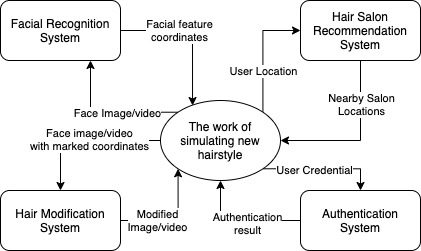
\includegraphics[width=\textwidth]{system_context_diagram}
\begin{figure}[h!]
\begin{center}
 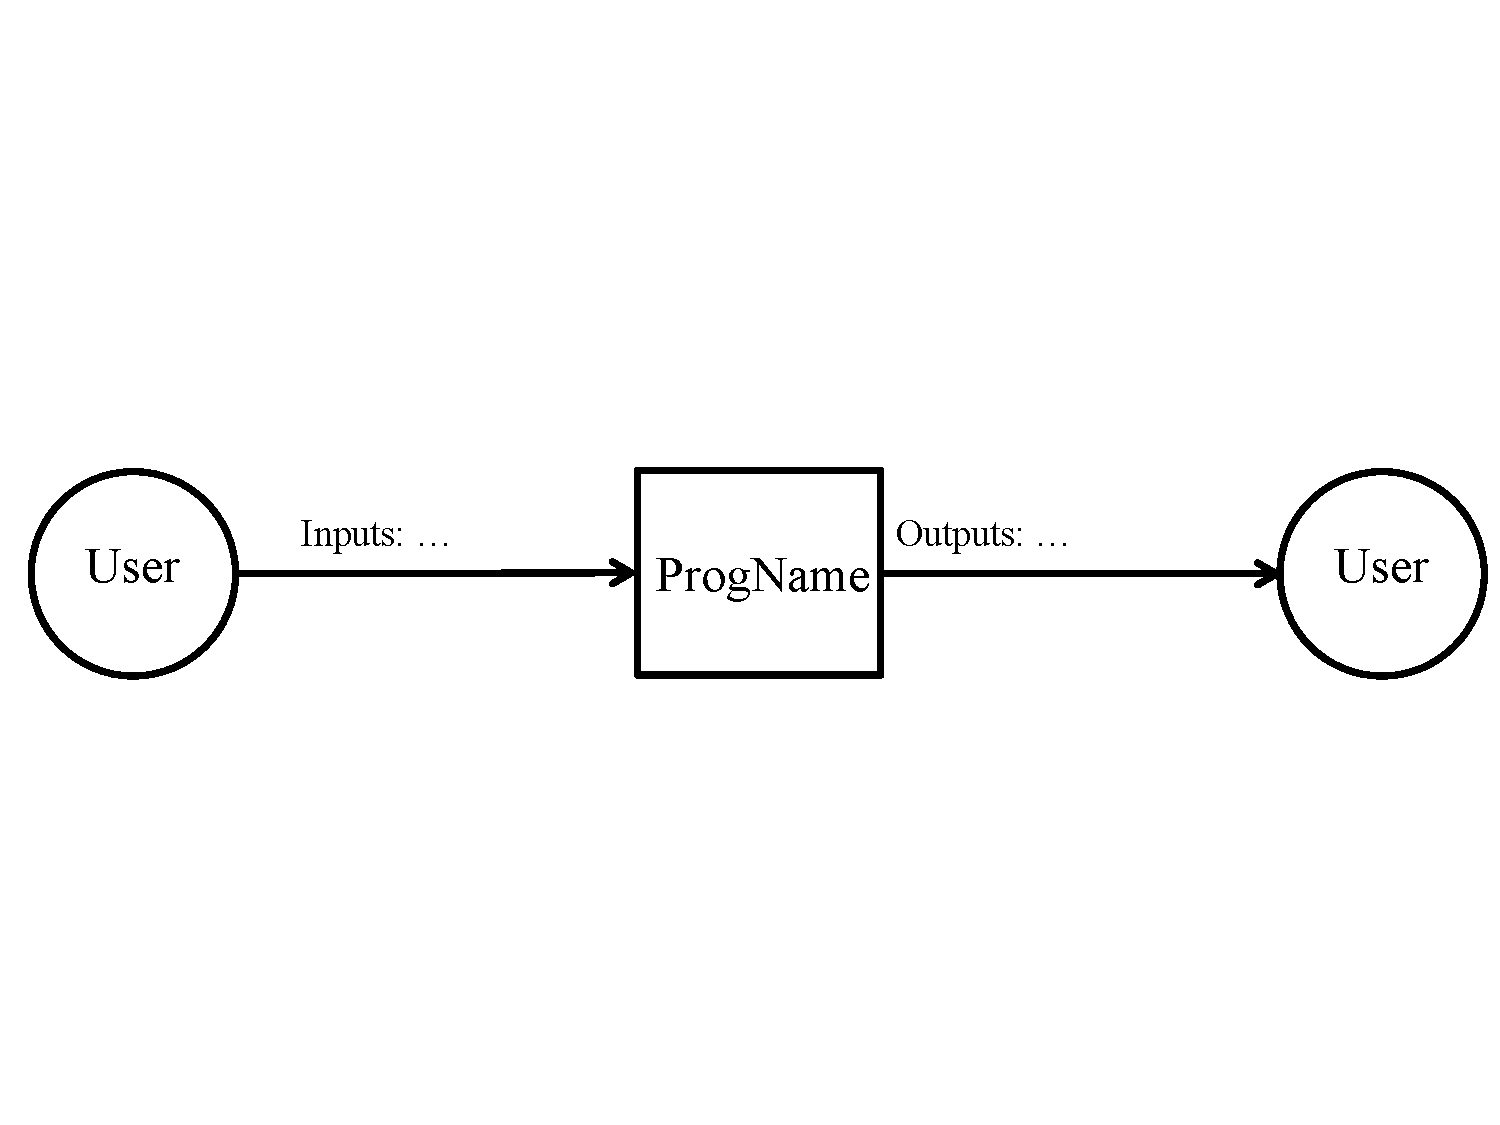
\includegraphics[width=0.6\textwidth]{SystemContextFigure}
\caption{Context of System Diagram}
\end{center}
\end{figure}

\subsection{Functional Requirements }
\subsubsection{Facial Recognition System}
    \begin{itemize}
        \item[FR\refstepcounter{frreqnum}\thefrreqnum \label{R_Inputs}:] The user must input their face in image or video format
        \item[FR\refstepcounter{frreqnum}\thefrreqnum \label{R_Inputs}:] The system must pre-process the image by transforming the input facial image to grayscale
        \item[] Rationale: Increase the contrastness of the image to better detect the edges
        \item[] Math Specification: newImage $:=$ process($image$) $\Rightarrow$ ($\forall p :$ Pixels in image $|$ p[$Red$]*0.21 + p[$Green$]*0.72 + p[$Blue$]*0.07)
        \item[FR\refstepcounter{frreqnum}\thefrreqnum \label{R_Inputs}:] The system must load the grayscale facial image into a pre-trained facial detection model for face shape detection
        \item[] Rationale: The pre-trained facial detection model needs a grayscale image as an input to provide a more accurate result
        \item[FR\refstepcounter{frreqnum}\thefrreqnum \label{R_Inputs}:] The system must load the pre-processed image into a pre-trained hair detection model for hair extraction
        \item[] Rationale: The pre-trained hair detection model needs a grayscale image as an input to provide a more accurate result
        \item[FR\refstepcounter{frreqnum}\thefrreqnum \label{R_Inputs}:] The system compute the hair edge coordinates
        \item[] Rationale: the pre-trained models will compute a series of important coordinates related to the hair. These coordinates will be used for various transformation.
        \item[FR\refstepcounter{frreqnum}\thefrreqnum \label{R_Inputs}:] The system must mark the corners and shape with facial landmark coordinates.
        \item[] Rationale: Marking the boundary is important, because the transformations will only apply to the hair not the face.
        \item[FR\refstepcounter{frreqnum}\thefrreqnum \label{R_Inputs}:] The system must store the coordinates from the hair and facial features.
    \end{itemize}

\subsubsection{Hair Modification System}
    \begin{itemize}
        \item[HM\refstepcounter{hmreqnum}\thehmreqnum \label{R_Inputs}:] The user must choose a color from the provided options if hair color transformation is selected
        \item[HM\refstepcounter{hmreqnum}\thehmreqnum \label{R_Inputs}:] The system must load the hair feature data for hair color transition
        \item[HM\refstepcounter{hmreqnum}\thehmreqnum \label{R_Inputs}:] The system should map the hair coordinates on the image and apply the new rgb values to the region
        \item[] Rationale: The hair coordinates are retrieved from facial recognition system, so new rgb colors can be applied to those regions
        \item[HM\refstepcounter{hmreqnum}\thehmreqnum \label{R_Inputs}:] The system must load the facial coordinates for hair style transformation
        \item[HM\refstepcounter{hmreqnum}\thehmreqnum \label{R_Inputs}:] The user must choose a hair style from the provided options if hair style transformation is selected
        \item[HM\refstepcounter{hmreqnum}\thehmreqnum \label{R_Inputs}:] The system should load the selected hair style dataset from the database
        \item[HM\refstepcounter{hmreqnum}\thehmreqnum \label{R_Inputs}:] the system should adjust the coordinate to be proportional with the image scale
        \item[HM\refstepcounter{hmreqnum}\thehmreqnum \label{R_Inputs}:] The system should add the new hair style coordinates above the facial coordinates.
        \item[] Rationale: depends on the hair style, some can be placed on top of the existing hair style, or re-construct
        \item[HM\refstepcounter{hmreqnum}\thehmreqnum \label{R_Inputs}:] The system should output the transformed face in image or video.
    \end{itemize}
\subsubsection{Hair Salon Recommendation System}
    \begin{itemize}
        \item[HR\refstepcounter{hrreqnum}\thehrreqnum \label{R_Inputs}:] The user must enter a address or turn on current location to use the recommendation system
        \item[HR\refstepcounter{hrreqnum}\thehrreqnum \label{R_Inputs}:] The system must retrieve 5 nearby hair salon locations based on the input address
        \item[HR\refstepcounter{hrreqnum}\thehrreqnum \label{R_Inputs}:] The system should label the retrieved locations on a map
        \item[] Rationale: marking the locations on the map allows the user to see the distance to their current location visually
        \item[HR\refstepcounter{hrreqnum}\thehrreqnum \label{R_Inputs}:] The system should rank the locations based on user review
        \item[] Rationale: the user reviews is a good indicator for deciding which one to go to
    \end{itemize}
    
\subsubsection{Authentication System}
    \begin{itemize}
        \item[AR\refstepcounter{arreqnum}\thearreqnum \label{R_Inputs}:] The user must enter valid username and password to access their profile in the system
        \item[AR\refstepcounter{arreqnum}\thearreqnum \label{R_Inputs}:] The system must allow the user to upload their face image before and after hair transformation
        \item[] Rationale: users might want to save the images for future references
        \item[AR\refstepcounter{arreqnum}\thearreqnum \label{R_Inputs}:] The system shall upload images after successful log in
        \item[AR\refstepcounter{arreqnum}\thearreqnum \label{R_Inputs}:] The system must allow the user to log out
    \end{itemize}

\subsection{Finite State Machine}
\graphicspath{ {./fsm.jpg/} }
\includegraphics[width=\textwidth]{FSM}
\begin{figure}[h!]
\begin{center}
 \includegraphics[width=0.8\textwidth]{FSMFigure}
\caption{Finite State Machine}
\end{center}
\end{figure}


\section{Nonfunctional Requirements}

\subsection{Look and Feel Requirements}
\subsubsection{Appearance Requirements}
\begin{itemize}
    \item[APR\refstepcounter{aprreqnum}\theaprreqnum \label{R_Inputs}:] The fonts must be outstanding and easily recognizable through the interface.
    \item[] Fit Criteria: Volunteers from various age ranges will be invited to verify that they can see the text with the application font size.
    \item[APR\refstepcounter{aprreqnum}\theaprreqnum \label{R_Inputs}:] The user interface should be well-organized while simple to use. 
    \item[] Fit Criteria: Volunteers from different age group will be invited to use the application and see if they can learn how to use by themselves. 
\end{itemize}

\subsubsection{Style Requirements}
\begin{itemize}
    \item[IAR\refstepcounter{iarreqnum}\theiarreqnum \label{R_Inputs}:] The style of the interface must has a modern aesthetic.
    \item[] Fit Criteria: The interface will be compared with the popular modern interface style found online. Professional UI Designers will be invited to take a look at the application interface to ensure the interface has a mordern aesthetic.
    \item[IAR\refstepcounter{iarreqnum}\theiarreqnum \label{R_Inputs}:] The style of the interface must be simple and clear. 
    \item[] Fit Criteria: Volunteers will be invited to use the application, and there should be no user reflects that the interface is complicated, unclear, and hard to use.
\end{itemize}
\subsection{Usability and Humanity Requirements}

\subsubsection{Ease of Use Requirements}
\begin{itemize}
    \item[EUR\refstepcounter{eurreqnum}\theeurreqnum \label{R_Inputs}:] Interactable components on the interface should be emphasized to signify the user that the components can be interacted with.
    \item[] Fit Criteria: Volunteers will be invited to use the application and see if they can intuitively find out all the interactable components.
    \item[EUR\refstepcounter{eurreqnum}\theeurreqnum \label{R_Inputs}:] Interactable components on the interface should be big enough to prevent the user from misclicking.
    \item[] Fit Criteria: Volunteers will be invited to use the application and see if they will misclick throughout using the application.
\end{itemize}

\subsubsection{Personalization and Internationalization Requirements}
N/A

\subsubsection{Learning Requirements}
\begin{itemize}
    \item[LR\refstepcounter{lrreqnum}\thelrreqnum \label{R_Inputs}:] The installation process must be completed within 3 steps.
    \item[LR\refstepcounter{lrreqnum}\thelrreqnum \label{R_Inputs}:] The instructions shall be concise and easy to follow.
    \item[] Fit Criteria: Volunteers will be invited to use the application and see if they can follow the instructions without problems.
\end{itemize}

\subsubsection{Understandability and Politeness Requirements}
\begin{itemize}
    \item[UPR\refstepcounter{uprreqnum}\theuprreqnum \label{R_Inputs}:] The icons should be taken from common usage icons when appropriate.
    \item[] Fit Criteria: Volunteers will be invited to use the application and see if all the icons make sense where they were used
\end{itemize}

\subsubsection{Accessibility Requirements}
\begin{itemize}
    \item[ASR\refstepcounter{asrreqnum}\theasrreqnum \label{R_Inputs}:] Fonts shall be in appropriate color and size
    \item[] Rationale: The content can be easily read by the user.
    \item[] Fit Criteria: Volunteers will be invited to use the application and rate the readability of the content from 1-10, below 7 is a fail.
\end{itemize}


\subsection{Performance Requirements}
\subsubsection{Speed and Latency Requirements}
\begin{itemize}
    \item[SLR\refstepcounter{slrreqnum}\theslrreqnum \label{R_Inputs}:] The response time of hairstyle suggestion must be within 1 second.
    \item[SLR\refstepcounter{slrreqnum}\theslrreqnum \label{R_Inputs}:] The response time of users changing hairstyles must be within 1 second.
    \item[SLR\refstepcounter{slrreqnum}\theslrreqnum \label{R_Inputs}:] The response time of users clicking any other buttons must be within 0.5 seconds.
\end{itemize}

\subsubsection{Safety-Critical Requirements}
N/A

\subsubsection{Precision and Accuracy Requirements}
\begin{itemize}
    \item[PAR\refstepcounter{parreqnum}\theparreqnum \label{R_Inputs}:] The position of the AR hair must fit the users' head position on the screen within 1 millimeter accuracy.
    \item[PAR\refstepcounter{parreqnum}\theparreqnum \label{R_Inputs}:] When users move their heads, the AR hair must move along the users' heads within 2 millimeters accuracy.
\end{itemize}

\subsubsection{Reliability and Availability Requirements}
\begin{itemize}
    \item[RAR\refstepcounter{rarreqnum}\therarreqnum \label{R_Inputs}:] For all users, the application will be available to use without crashes over 99 percents of the time. (less than or equal to 1 crash per 100 access)
    \item[RAR\refstepcounter{rarreqnum}\therarreqnum \label{R_Inputs}:] The application must allow the users to use continuously until the hardware device is broken or out of battery. 
    \item[] Fit Criteria: There should be no errors during unit tests, integration test and user tests for the application.
\end{itemize}

\subsubsection{Robustness Requirements}
\begin{itemize}
    \item[RBR\refstepcounter{rbrreqnum}\therbrreqnum \label{R_Inputs}:] The application must have exception handling methods to provide useful feedback if improper information is input.
    \item[] Fit Criteria: There should be a pressure test on the application and developers will try to inject irrational inputs to break the application, but no errors or exceptions should occur.
    \item[RBR\refstepcounter{rbrreqnum}\therbrreqnum \label{R_Inputs}:] The application must have error case handling methods so that it can recover from simple errors such as stuck or no response.
    \item[] Fit Criteria: There should be a pressure test on the application and developers will try to inject irrational inputs to break the application, but the application should not crash.
\end{itemize}

\subsubsection{Capacity Requirements}
\begin{itemize}
    \item[CCR\refstepcounter{ccrreqnum}\theccrreqnum \label{R_Inputs}:] The application must have a database to store every user's account information.
    \item[] Fit Criteria: Database developer will do tests on the database such that the count of users' account information in the database equals the actual registered number of user accounts.
    \item[CCR\refstepcounter{ccrreqnum}\theccrreqnum \label{R_Inputs}:] The product must have a database to store at least 10 different hairstyles.
\end{itemize}

\subsubsection{Scalability and Extensibility Requirements}
\begin{itemize}
    \item[SER\refstepcounter{serreqnum}\theserreqnum \label{R_Inputs}:] The application must allow new features to be added in the future.
    \item[] Fit Criteria: Any possible future developing features will be kept in the section of Watch Room in this document.
\end{itemize}

\subsubsection{Longevity Requirements}
\begin{itemize}
    \item[LGR\refstepcounter{lgrreqnum}\thelgrreqnum \label{R_Inputs}:] The application must be supported while the libraries and frameworks being used are supported and all developers constantly maintaining.
    \item[] Fit Criteria: Developers will regularly run tests to ensure the application is functioning.
\end{itemize}

\subsection{Operational and Environmental Requirements}
\subsubsection{Expected Physical Environment}
N/A

\subsubsection{Requirements for Interfacing with Adjacent System}
N/A

\subsubsection{Productization Requirements}
\begin{itemize}
    \item[PDR\refstepcounter{pdrreqnum}\thepdrreqnum \label{R_Inputs}:] The product must be available to download via Apple App Store.
    \item[] Fit Criteria: Volunteers and developers will search and download the application via Apple App Store and all people should download the application successfully.
\end{itemize}

\subsubsection{Release Requirements}
\begin{itemize}
    \item[RER\refstepcounter{rerreqnum}\thererreqnum \label{R_Inputs}:] Data from previous builds of the product should be compatible with new builds of the product.
    \item[] Fit Criteria: Developers will regularly run tests to ensure that data can be used between different builds.
    \item[RER\refstepcounter{rerreqnum}\thererreqnum \label{R_Inputs}:] Version updates and descriptions of changes shall be included in change logs available to the user.
\end{itemize}

\subsection{Maintainability and Support Requirements}
\subsubsection{Maintenance Requirements}
\begin{itemize}
    \item[MSR\refstepcounter{msrreqnum}\themsrreqnum \label{R_Inputs}:] 
    The product will be maintained by the developers.
    \item[] Fit Criteria: Developers will regularly run tests and fix bugs if any occur.
    \item[MSR\refstepcounter{msrreqnum}\themsrreqnum \label{R_Inputs}:] 
    The product shall undergo revision to check for any potential bugs.
    \item[] Fit Criteria: Developers will regularly run tests to check for potential bugs.
    \item[MSR\refstepcounter{msrreqnum}\themsrreqnum \label{R_Inputs}:] 
    The mean time to restore the App (MTTRS) following a system failure must not be greater than 60 minutes. MTTRS includes all corrective maintenance time and delay time
\end{itemize}
\subsubsection{Supportability Requirements}
\begin{itemize}
    \item[SPR\refstepcounter{sprreqnum}\thesprreqnum \label{R_Inputs}:] 
    The product shall be available on iPhone with iOS system 14 and after.
    \item[] Volunteers with iPhone 
\end{itemize}

\subsubsection{Adaptablity Requirements}
\begin{itemize}
    \item[ADR\refstepcounter{adrreqnum}\theadrreqnum \label{R_Inputs}:] 
    The product shall be compatible with iOS system 14 and after.
    
\end{itemize}

\subsection{Security Requirements}

\subsubsection{Access Requirements}
\begin{itemize}
    \item[ACR\refstepcounter{acrreqnum}\theacrreqnum \label{R_Inputs}:] Users will be able to access images they previously stored.
    \item[] Fit Criteria: Developers will run tests as user role to ensure that stored data is accessible.
    \item[ACR\refstepcounter{acrreqnum}\theacrreqnum\label{R_Inputs}:] 
    Users will be able to access site data for job sites they are authorized for.
    \item[] Fit Criteria: Developers will run tests in user role to ensure that data is accessible with permission.
    \item[ACR\refstepcounter{acrreqnum}\theacrreqnum \label{R_Inputs}:]
    Admins and supervisors will be able to unlock locked resources.
    \item[] Fit Criteria: Developers will run tests in admin role to ensure that locked resources are accessible to admins and supervisors.
    \item[ACR\refstepcounter{acrreqnum}\theacrreqnum \label{R_Inputs}:]
    Only admins will be able to modify application information.
    \item[] Fit Criteria: Developers will run tests in admin role to ensure that only admins can modify application information.
\end{itemize}


\subsubsection{Integrity Requirements}
\begin{itemize}
    \item[IR\refstepcounter{irreqnum}\theirreqnum \label{R_Inputs}:] The product will not modify data unnecessary.
    \item[] Fit Criteria: Developers will run tests in a sandbox to verify that data is only modified when necessary.
    \item[IR\refstepcounter{irreqnum}\theirreqnum \label{R_Inputs}:] The product will not modify any data unrelated to its execution.
    \item[] Fit Criteria: Developers will run tests in a sandbox to verify that data is only modified when it is related to its execution.
    \item[IR\refstepcounter{irreqnum}\theirreqnum \label{R_Inputs}:] Data will be automatically backed up daily.
     \item[] Fit Criteria: Developers will verify that the cloud database is backed up daily.
    \item[IR\refstepcounter{irreqnum}\theirreqnum \label{R_Inputs}:] Unsaved data will be stored locally on the user's device if it cannot be uploaded to the remote database and is not explicitly discarded.
    \item[] Fit Criteria: Developers will run tests in user role to ensure that unsaved data is stored locally on the user's device if it cannot be uploaded to the remote database and is not explicitly discarded.
\end{itemize}

\subsubsection{Privacy Requirements}
\begin{itemize}
    \item[PRR\refstepcounter{prrreqnum}\theprrreqnum \label{R_Inputs}:] Users will not be able to access data generated by other users.
    \item[] Fit Criteria: Developers will run tests in user role to ensure that users cannot access data generated by other users.
    \item[PRR\refstepcounter{prrreqnum}\theprrreqnum \label{R_Inputs}:] Users will be required to register and login to the application with their emails.
    \item[] Fit Criteria: Developers will run tests in user role to ensure that users cannot access data generated by other users.
\end{itemize}

\subsubsection{Audit Requirements}
\begin{itemize}
    \item[AUR\refstepcounter{aurreqnum}\theaurreqnum \label{R_Inputs}:] Requirements should be easy to read and verify against the system facilitate regular inspections.
    \item[] Fit Criteria: SRS requirements will be verified by SE4G06A teaching assistants.
\end{itemize}

\subsubsection{Immunity Requirements}
N/A

\subsection{Cultural and Political Requirements}
\subsubsection{Cultural Requirements}
\begin{itemize}
    \item[CR\refstepcounter{crreqnum}\thecrreqnum \label{R_Inputs}:] The product will not use any terms that are inappropriate or offensive towards any cultures.
    \item[] Fit Criteria: Volunteers will be invited to use the application and see if they find any inappropriate terms.
\end{itemize}

\subsubsection{Political Requirements}
N/A

\subsection{Legal Requirements}
\subsubsection{Compliance Requirements}
\begin{itemize}
    \item[CPR\refstepcounter{cprreqnum}\thecprreqnum \label{R_Inputs}:] The product must state that the application does not take responsibility for any accidents resulting from its use. 
\end{itemize}

\subsubsection{Standards Requirements}
\begin{itemize}
    \item[SDR\refstepcounter{sdrreqnum}\thesdrreqnum \label{R_Inputs}:] The product must follow the fail-safe-defaults design principle in that it will always error into a safe state.
    \item[SDR\refstepcounter{sdrreqnum}\thesdrreqnum \label{R_Inputs}:] The product must follow modular design principles to allow for easy maintenance.
    \item[SDR\refstepcounter{sdrreqnum}\thesdrreqnum \label{R_Inputs}:] The application must be developed using iOS application style guides. 

\end{itemize}

\subsubsection{Health and Safety Requirements}
N/A

\section{Likely Changes}    

\noindent \begin{itemize}

\item[LC\refstepcounter{lcnum}\thelcnum\label{LC_meaningfulLabel}:] 
This project will only result in the development of a mobile iOS app. However, an android application may also be developed to work with, or in place of, the iOS application in the future.
\item[LC\refstepcounter{lcnum}\thelcnum\label{LC_meaningfulLabel}:] 
The application may be extended to offer compatibility as a web application.
\item[LC\refstepcounter{lcnum}\thelcnum\label{LC_meaningfulLabel}:] 
The application will not initially pursue functionality for users to "cut" their 3D simulated hair.
\item[LC\refstepcounter{lcnum}\thelcnum\label{LC_meaningfulLabel}:] 
The application may require more data for the facial recognition feature.
\item[LC\refstepcounter{lcnum}\thelcnum\label{LC_meaningfulLabel}:] 
The load capacity of the system is initially set low for the first edition of this application. As demand for the application increases, the load capacity must also increase to support a larger user base.
\item[LC\refstepcounter{lcnum}\thelcnum\label{LC_meaningfulLabel}:] 
The application may be required to include new features as discovered through use of the system in real-world scenarios.
\item[LC\refstepcounter{lcnum}\thelcnum\label{LC_meaningfulLabel}:] 
The format of the
input and output data of facial recognition, hair modification, hair salon recommendation system.
\item[LC\refstepcounter{lcnum}\thelcnum\label{LC_meaningfulLabel}:] 
The interface style requirements might change since no metric has been provided for this by stakeholders. 
\item[LC\refstepcounter{lcnum}\thelcnum\label{LC_meaningfulLabel}:] 
The speed and latency requirements might change since no metric has been provided for this by stakeholders. 
\item[LC\refstepcounter{lcnum}\thelcnum\label{LC_meaningfulLabel}:] 
The precision and accuracy requirements might change since no metric has been provided for this by stakeholders. 




\end{itemize}

\section{Unlikely Changes}    

\noindent \begin{itemize}

\item[ULC\refstepcounter{ulcnum}\theulcnum\label{ULC_meaningfulLabel}:] 
Since several of the features might require exposing API endpoints, an offline-only version of the application is unlikely to be necessary. 
\item[ULC\refstepcounter{ulcnum}\theulcnum\label{ULC_meaningfulLabel}:] 
As the main demographic of this application is less computer literate, the ease of use of this application must remain a high priority consideration throughout the design of this system.
\item[ULC\refstepcounter{ulcnum}\theulcnum\label{ULC_meaningfulLabel}:] 
The application is designed to ensure that data will only be modified when necessary. 
\item[ULC\refstepcounter{ulcnum}\theulcnum\label{ULC_meaningfulLabel}:] 
The application is designed to ensure that only admins and supervisors will be able to unlock locked resources.
\item[ULC\refstepcounter{ulcnum}\theulcnum\label{ULC_meaningfulLabel}:] 
The application is designed to ensure that no inappropriate or offensive language towards any culture will be used.
\item[ULC\refstepcounter{ulcnum}\theulcnum\label{ULC_meaningfulLabel}:] 
The application is designed to ensure compliance with the Data Privacy Act of Canada. All user personal information will not be stored or used without consent. 
\item[ULC\refstepcounter{ulcnum}\theulcnum\label{ULC_meaningfulLabel}:] 
The application is designed to ensure that users are only able to see data that they have proper authorization for.
\item[ULC\refstepcounter{ulcnum}\theulcnum\label{ULC_meaningfulLabel}:] 
The application is designed to help users simulate hairstyles and hair colors virtually.
\item[ULC\refstepcounter{ulcnum}\theulcnum\label{ULC_meaningfulLabel}:] 
The primary user of this project is unlikely going to change since the project purpose is determined already, only certain types of users will be interested in this kind of application.
\item[ULC\refstepcounter{ulcnum}\theulcnum\label{ULC_meaningfulLabel}:] 
The client of this project is unlikely going to change because this project is a student capstone project and it has limited marketability.
\item[ULC\refstepcounter{ulcnum}\theulcnum\label{ULC_meaningfulLabel}:] 
The schedule and budget constraints are not likely going to change, because this project is a student capstone project. It needs to strictly follow SE4G06 course constraints.








\end{itemize}

\bibliographystyle {plainnat}
\bibliography {../../refs/References}

\section{Project Issues}

\subsection{Open Issues}
One of the issues is that the team does not have sufficient background knowledge in technologies we are going to use: AR, Computer Vision, and iOS development. Developers must learn these technologies before implementation of the application.


\subsection{Off-the-Shelf Solutions}
Until now, there are a few similar open source projects online for us to go through. Since they are all written in different coding styles and design structures, we will only be gathering the basic concepts from these projects. Besides, to ensure that everyone in our team will be at the same pace and participate in the actual project, everyone in our team will take some time to play around with ARkit and swift before getting our hands on the actual design.

\subsection{New Problems}
\subsubsection{Effects on current environment}
\begin{enumerate}
    \item The application will occupy the camera of the iOS mobile system when the application runs, and other applications in the same system can not use the camera function during this time.
    \item The application will occupy some memory in the iOS mobile system for it to run.
\end{enumerate}

\subsubsection{Potential User Problem}
\begin{enumerate}
    \item Since pictures of users' faces will be saved in the system database,
    any potential data breach will exposes user privacy. 
    \item If the user uses the application under strong sunlight or in a dark environment, the user can potentially damage the eyes.
    \item If the user uses the application when crossing traffics, there is a potential of traffic accident.
\end{enumerate}

\subsubsection{Limitations in the Anticipated Implementation Environment That May Inhibit the New Product}
\begin{enumerate}
    \item The back-end server may not be powerful enough to handle high volume of requests from users.
    \item The size of the application may be too large to install in a normal iOS mobile.
\end{enumerate}

\subsubsection{Follow-Up Problems}
\begin{enumerate}
    \item Will we create a demand for our product that we are not able to service?
    \item Will the new system cause us to run afoul of laws that do not currently apply?
    \item Will the existing hardware on users' iOS mobile cope?
\end{enumerate}
\newpage
\subsection{Tasks}
\begin{flushleft}
\begin{table}[bp hp]
\caption{\bf Phase In Plan}
    \begin{tabularx}{\linewidth}{|l|X|}
        \toprule {\bf Task} & {\bf Timeline}\\
        \midrule
        Discuss \& Revise requirements  & Oct 5th\\
        \hline
        Submit SRS & Oct 5th\\
        \hline
        Initial Draft of Hazard Analysis & Oct 12th\\
        \hline
        Revision of Hazard Analysis & Oct 18th\\
        \hline
        Submit Hazard Analysis & Oct 19th\\
        \hline
        Initial Draft of VnV Plan & Oct 24th\\
        \hline
        Revision of VnV Plan & Nov 1nd\\
        \hline
        Submit VnV Plan & Nov 2nd\\
        \bottomrule
    \end{tabularx}
\end{table}
\end{flushleft}

\begin{flushleft}
\begin{table}[bp hp]
\caption{\bf Project Implementation Tasks}
    \begin{tabularx}{\linewidth}{|l|X|}
        \toprule {\bf Task Name} & {\bf Description}\\
        \midrule
        Implement basic UI & An iOS UI that can access the camera and get camera inputs and pass it to back end\\
        \hline
        Implement Computer Vision & A component in the back end that receives camera inputs and use computer vision technique to analyze human face and output to the front end\\
        \hline
        Implement AR functionality in UI & A component in the front end that takes the analyzed output from computer vision in backend and apply AR technique to add hairs on the user's face on the screen\\
        \hline
        Implement Database & A database to store user information\\
        \hline
        Implement Database interaction on UI & Add a component to fulfill read and write access to database\\
        \bottomrule
    \end{tabularx}
\end{table}
\end{flushleft}
\subsection{Migration to the New Product}
N/A

\subsection{Risks}
Some of the testing process will be difficult to automate, since the product will need actual human to judge whether the hairstyle fits smoothly on the 3D model. For this part of the testing, we will draw random samples and ask people around us to perform physical testing.

\subsection{Costs}

Other than the time it takes to develop the application there might be a cost for using some licensed libraries. 

\subsection{User Documentation and Training}
\subsubsection{User Documentation Requirements}
\begin{enumerate}
    \item A readme file will be provided in the documentation for user to read. The file will provide a full guideline of how to install and use our application.
    \item A technical specification will be provided for other developers who would like to make further changes to our application.
    \item The guideline will also be available on the help page of the running application.
\end{enumerate}
\subsubsection{Training Requirements}
N/A

\subsection{Waiting Room}

The application shall allow users to cut and make changes to their hairstyles, in order to enhance user experiences.

\subsection{Ideas for Solutions}
\begin{itemize}
    \item Add function in computer vision to capture user hand gestures, with the specific gesture motion on a specific area of hair, the hair beneath the hand will be cut.
\end{itemize}

\section{Traceability Matrix}

\begin{landscape}
\begin{table}[h!]
\centering
\begin{tabular}{|c|c|c|c|c|c|c|c|c|c|c|c|c|c|c|c|c|}
\hline
	& FR1 & FR2 & FR3 & FR4 & FR5 & FR6 & FR7 & HM1 & HM2 & HM3 & HM4 & HM5 & HM6 & HM7 & HM8 & HM9 \\
\hline
APR1        & & & & & & & & & & & & & & & & \\ \hline
APR2        & & & & & & & & & & & & & & & &  \\ \hline
IAR1        & & & & & & & & & & & & & & & & \\ \hline
IAR2        & & & & & & & & & & & & & & & & \\ \hline
EUR1        &X & & &X &X & &X & & & & & & & & & \\ \hline
EUR2        & &X &X & &X & &X & & & & & & & & & \\ \hline
LR1         & & & & & & & & & & & & & & & & \\ \hline
LR2         & & & & & & & & & & & & & & & & \\ \hline
UPR1        & & & & & & & & & & & & & & & & \\ \hline
ASR1        & & & & & & & & & & & & & & & & \\ \hline
SLR1        & X& & & & & & & & & & & X& & X& & \\ \hline
SLR2        & & & & & & & & & & & & X& & X& X& \\ \hline
SLR3        & & & & & & & & & & X& & X& & & X& \\ \hline
PAR1        & & & & & & & & & & & X& & X& & & \\ \hline
PAR2        & & & & & & & & & & & & X& & X& & \\ \hline
RAR1        & & & & & & & & & & & & & & & & \\ \hline
RAR2        & & & & & & & & & & & & & & & & \\ \hline
RBR1        & & & & & & & & & & & & & & & & \\ \hline
RBR2        & & & & & & & & & & & & & & & & \\ \hline
CCR1        & & & & & & & & & & & & & & & & \\ \hline
CCR2        & & & & & & & & & & & & & & & & \\ \hline
SER1        & & & & & & & & & & & & & & & & \\ \hline
LGR1        & & & & & & & & & & X & & & X& & & \\ \hline
PDR1        & & & & & & & & & & & & & & & & \\ \hline
RER1        & & & & & & & & & & & & & & & & \\ \hline

\end{tabular}
\caption{Traceability Matrix Showing the Connections Between Functional Requirements and Non-functional Requirements}
\label{Table:A_trace}
\end{table}
\end{landscape}

\begin{landscape}
\begin{table}[h!]
\centering
\begin{tabular}{|c|c|c|c|c|c|c|c|c|c|c|c|c|c|c|c|c|}
\hline
	& FR1 & FR2 & FR3 & FR4 & FR5 & FR6 & FR7 & HM1 & HM2 & HM3 & HM4 & HM5 & HM6 & HM7 & HM8 & HM9 \\
\hline
RER2        & & & & & & & & & & & & & & & & \\ \hline
MSR1        & & & & & & & & & & & & & & & & \\ \hline
MSR2        & & & & & & & & & & & & & & & & \\ \hline
MSR3        & & & & & & & & & & & & & & & & \\ \hline
ADR1        & & & & & & & & & & & & & & & & \\ \hline
ACR1        & & & & & & & & & & & & & & & & \\ \hline
ACR2        & & & & & & & & & & & & & & & & \\ \hline
ACR3        & & & & & & & & & & & & & & & & \\ \hline
ACR4        & & & & & & & & & & & & & & & & \\ \hline
IR1         & & & & & & & & & & & & & & & & \\ \hline
IR2         & & & & & & & & & & & & & & & & \\ \hline
IR3         & & & & & & & & & & & & & & & & \\ \hline
IR4         & & & & & & & & & & & & & & & & \\ \hline
PRR1        & & & & & & & & & & & & & & & & \\ \hline
PRR2        & & & & & & & & & & & & & & & & \\ \hline
AUR1        & & & & & & & & & & & & & & & & \\ \hline
CR1         & & & & & & & & & & & & & & & & \\ \hline
CPR1        & & & & & & & & & & & & & & & & \\ \hline
SDR1        & & & & & & & & & & & & & & & & \\ \hline
SDR2        & & & & & & & & & & & & X & & & & \\ \hline
SDR3        & & & & & & & & & & & & & & & & \\ \hline
RER1        & & & & & & & & & & & & & & & & \\ \hline

\end{tabular}
\caption{Traceability Matrix Showing the Connections Between Functional Requirements and Non-functional Requirements}
\label{Table:A_trace}
\end{table}
\end{landscape}

\begin{landscape}
\begin{table}[h!]
\centering
\begin{tabular}{|c|c|c|c|c|c|c|c|c|}
\hline
& HR1 & HR2 & HR3 & HR4 & AR1 & AR2 & AR3 & AR4 \\
\hline
APR1        & & & & & & & & \\ \hline
APR2        & & & & & & & & \\ \hline
IAR1        & & & & & & & & \\ \hline
IAR2        & & & & & & & & \\ \hline
EUR1        &X &X & & & & & & \\ \hline
EUR2        &X & &X &X & & & & \\ \hline
LR1         & & & & & & & & \\ \hline
LR2         & & & & & & & & \\ \hline
UPR1        & & & & & & & & \\ \hline
ASR1        & & & & & & & & \\ \hline
SLR1        & & & & & & & & \\ \hline
SLR2        & & & & & & & & \\ \hline
SLR3        & & & & & & & & \\ \hline
PAR1        & & & & & & & & \\ \hline
PAR2        & & & & & & & & \\ \hline
RAR1        & & & & & & & & \\ \hline
RAR2        & & & & & & & & \\ \hline
RBR1        & & & & & & & & \\ \hline
RBR2        & & & & & & & & \\ \hline
CCR1        & & & & & & & & \\ \hline
CCR2        & & & & & & & & \\ \hline
SER1        & & & & & & & & \\ \hline
LGR1        & & & & & & & & \\ \hline
PDR1        & & & & & & & & \\ \hline
RER1        & & & & & & & & \\ \hline
\end{tabular}
\caption{Traceability Matrix Showing the Connections Between Functional Requirements and Non-functional Requirements - Continue}
\label{Table:A_trace}
\end{table}
\end{landscape}

\begin{landscape}
\begin{table}[h!]
\centering
\begin{tabular}{|c|c|c|c|c|c|c|c|c|}
\hline
& HR1 & HR2 & HR3 & HR4 & AR1 & AR2 & AR3 & AR4 \\
\hline
RER2        & & & & & & & & \\ \hline
MSR1        & & & & & & & & \\ \hline
MSR2        & & & & & & & & \\ \hline
MSR3        & & & & & & & & \\ \hline
SPR1        & & & & & & & & \\ \hline
ADR1        & & & & & & & & \\ \hline
ACR1        & & & & & &X & & \\ \hline
ACR2        & & & & &X &X &X &X \\ \hline
ACR3        & & & & &X &X & &X \\ \hline
ACR4        & & & & &X &X & & \\ \hline
IR1         & & & & & & & & \\ \hline
IR2         & & & & & & & & \\ \hline
IR3         & & & & & & & & \\ \hline
IR4         & & & & & & & & \\ \hline
PRR1        & & & & & & & & \\ \hline
PRR2        & & & & & & & & \\ \hline
AUR1        & & & & & & & & \\ \hline
CR1         & & & & & & & & \\ \hline
CPR1        & & & & & & & & \\ \hline
SDR1        & & & & & & & & \\ \hline
SDR2        & & & & & & & & \\ \hline
SDR3        & & & & & & & & \\ \hline
\end{tabular}
\caption{Traceability Matrix Showing the Connections Between Functional Requirements and Non-functional Requirements - Continue}
\label{Table:A_trace}
\end{table}
\end{landscape}

\section*{Appendix --- References}

\begin{itemize}
    \item templates: https://gitlab.cas.mcmaster.ca/smiths/pub/-/blob/master/VolereTemplate16.doc
    \item J. Cook, “Converting color to grayscale,” John D. Cook — Applied Mathematics Con-sulting, 29-Apr-2019. [Online]. Available: \newline https://www.johndcook.com/blog/2009/08/24/algorithms-convert-color-grayscale/.
    \item Inc., A. (n.d.). Designing for IOS. Designing for iOS - Platforms - Human Interface Guidelines - Design - Apple Developer. \newline Retrieved October 5, 2022, from https://developer.apple.com/design/human-interface-guidelines/platforms/designing-for-ios/ 
\end{itemize}

\section*{Appendix --- Reflection}

The information in this section will be used to evaluate the team members on the
graduate attribute of Lifelong Learning.  Please answer the following questions:

\begin{enumerate}
  \item What knowledge and skills will the team collectively need to acquire to
  successfully complete this capstone project?  Examples of possible knowledge
  to acquire include domain-specific knowledge from the domain of your
  application, or software engineering knowledge, mechatronics knowledge or
  computer science knowledge.  Skills may be related to technology, or writing,
  or presentation, or team management, etc.  You should look to identify at
  least one item for each team member.\\ \\
  Upon completing your project, all members will learn more about writing software development documentation and prototype presentation. In this project, ARkit is a new tool for everyone. As a result, after completing this project, we all should be familiar with the technical knowledge which can help us to build more AR-related applications. 
  
  Although Charlotte and Senni had some prior experience with swift, this project will be their first time developing a serious iOS application, not only will they have the opportunity to implement application UI/UX, but they will also learn more about swift which will help them gain insights about iOS/mobile application development. Although Jack had some experience with database development, such as using SQL and MATLAB, this is the first time he take the challenge to deal with project-related data. For sure he will also become better at data processing after this project. Last but not least, Marlon, Hongwei and Bill will be the pioneers to adventure machine learning using OpenCV with regard to facial recognition detection. They will learn about many machine learning concepts. During the whole development, all team members will also share their knowledge about the new technology they have learnt to help each other become better engineers, and also the things they already know to help each other during the development. Besides, all members will practice the design pattern we have learned in previous years and improve our leadership, communication and cooperation skills.
  \item For each of the knowledge areas and skills identified in the previous
  question, what are at least two approaches to acquiring the knowledge or
  mastering the skill?  Of the identified approaches, which will each team
  member pursue, and why did they make this choice?
  \begin{enumerate}
  \item For swift programming learning. The first approach will be gathering information from a book called "Develop In Swift". And applying the knowledge they learned to our project will help them to master Swift. The second approach would be from the other team members who had some knowledge about it. In this way, Senni and Charlotte will get familiar with the basic syntax in a short time. 
  \item For database developing, Jack will be adventuring pandas from python and following the tutorial online to learn the basic functions of it. After that, he will also learn from the actual developing process to put the knowledge into physical development.
  \item For back end and AR developers, they will first go through a few examples on github to get the basic concept about how to use a machine learning model. And then during the actual project building, they will also learn along the development and gather all the information needed to build a successful AR platform. 
  \item For teamwork skills mentioned above, we will first take turns to be the leader and host the weekly meetings during the development. Besides, we will also follow an agile standard during the development to enhance our teamwork and cooperation skills.
  \end{enumerate}
\end{enumerate}

\end{document}